\documentclass{article}
\usepackage[T1]{fontenc}
\usepackage{lmodern}
\usepackage{anyfontsize}
\usepackage{graphicx} 
\usepackage[absolute,overlay]{textpos}
\setlength{\parindent}{0pt}
\usepackage{geometry}
\geometry{top=1in, bottom=1in, right=1in, left=1in}
\usepackage{multicol}
\usepackage{multirow}
\usepackage[pages=some]{background}
\usepackage{booktabs}

\usepackage{listings}
\usepackage{xcolor}

\usepackage{tikz}
\usetikzlibrary{automata, positioning}

\pagestyle{empty}

\backgroundsetup{
  scale=1,
  opacity=1,
  angle=0,
  contents={
\includegraphics[width=\paperwidth,height=\paperheight]{imagenes/portada.jpg}}
}

\definecolor{rojo}{rgb}{0.8, 0, 0}

\usepackage{titlesec}

\titleformat{\section}
  {\color{rojo}\Large\bfseries}
  {}
  {0pt}
  {}

\titleformat{\subsection}
  {\color{rojo}\large\bfseries}
  {}
  {0pt}
  {}

\begin{document}
\BgThispage\-
\begin{textblock*}{15cm} (4cm, 9cm)
    {\fontsize{22pt}{13pt}\selectfont
    \textcolor{rojo}{\textbf{REPORTE DE PRÁCTICA 2.2 \\AFD y AFND}}
    }
\end{textblock*}
\begin{textblock*}{15cm} (4cm, 11cm)
    {\fontsize{12pt}{16pt}\selectfont
    \textcolor{rojo}{\textbf{NOMBRE DE LA PRÁCTICA: \\Autómatas Finitos Deterministas y No Deterministas}}
    }
\end{textblock*}
\begin{textblock*}{15cm} (4cm, 13cm)
    {\fontsize{13pt}{16pt}\selectfont
    \textcolor{rojo}{\textbf{ALUMNO: ROCHA HERNANDEZ ROGELIO}}
    }
\end{textblock*}
\begin{textblock*}{15cm} (6cm, 14cm)
    {\fontsize{12pt}{16pt}\selectfont
    \textcolor{rojo}{\textbf{Dr. Eduardo Cornejo-Velázquez}}
    }
\end{textblock*}

\newpage

\section*{Ejercicio 1}
\textbf{Lenguaje:} Palabras sobre $\Sigma = \{0,1\}$ que inician en “0”. \\

\textbf{Tupla del AFD:} 
\begin{itemize}
    \item $\Sigma = \{0,1\}$
    \item $Q = \{q_0, q_1, q_2\}$
    \item $q_0$ es el estado inicial
    \item $F = \{q_1\}$
\end{itemize}

\textbf{Diagrama del AFD:}

\begin{center}
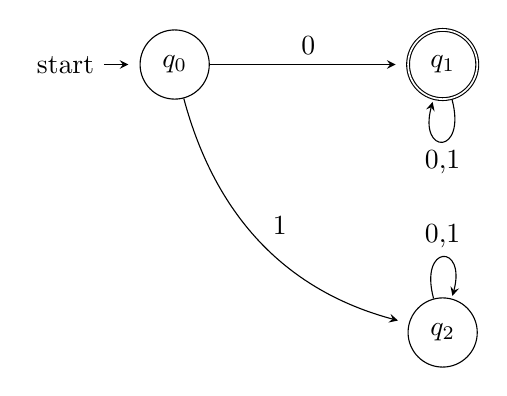
\begin{tikzpicture}[->, >=stealth, shorten >=4pt, auto, node distance=2.5cm]
% Estados
\node[state, initial] (q0) {$q_0$};
\node[state, accepting, right=of q0] (q1) {$q_1$};
\node[state, below=of q1] (q2) {$q_2$};
% Transiciones
\path
(q0) edge[above] node {0} (q1)
(q0) edge[bend right] node {1} (q2)
(q2) edge[loop above] node {0,1} ()
(q1) edge[loop below] node {0,1} ();
\end{tikzpicture}
\end{center}

\textbf{Tabla de transiciones:}

\begin{center}
\begin{tabular}{|c|c|c|}
\hline & 0 & 1   \\ \hline
$q_0$ & $q_1$ & $q_2$ \\ \hline
$q_1$ & $q_1$ & $q_1$ \\ \hline
$q_2$ & $q_2$ & $q_2$ \\ \hline
\end{tabular}
\end{center}

\textbf{Palabras aceptadas y palabras rechazadas}
\begin{center}
\begin{tabular}{|c|c|}
\hline
Aceptadas & No aceptadas \\
\hline
0 & 1 \\
01 & 10 \\
00 & 11 \\
000 & 101 \\
010 & 111 \\
\hline
\end{tabular}
\end{center}

\section*{Ejercicio 2}
\textbf{Lenguaje:} Palabras sobre $\Sigma = \{0,1\}$ que terminan en “1”. \\

\textbf{Tupla del AFD:}
\begin{itemize}
    \item $\Sigma = \{0,1\}$
    \item $Q = \{q_0, q_1\}$
    \item $q_0$ estado inicial
    \item $F = \{q_1\}$
\end{itemize}

\textbf{Diagrama del AFD:}

\begin{center}
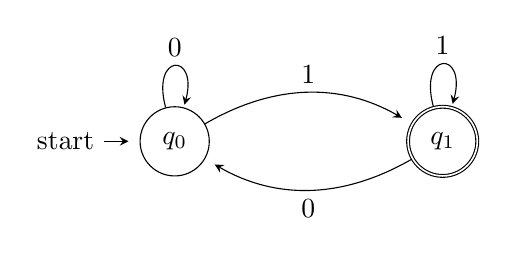
\begin{tikzpicture}[->, >=stealth, shorten >=4pt, auto, node distance=2.5cm]
% Estados
\node[state, initial] (q0) {$q_0$};
\node[state, accepting, right=of q0] (q1) {$q_1$};
% Transiciones
\path
(q0) edge[bend left] node {1} (q1)
(q1) edge[bend left] node {0} (q0)
(q0) edge[loop above] node {0} ()
(q1) edge[loop above] node {1} ();
\end{tikzpicture}
\end{center}

\textbf{Tabla de transiciones:}

\begin{center}
\begin{tabular}{|c|c|c|}
\hline
 & 0 & 1 \\ \hline
$q_0$ & $q_0$ & $q_1$ \\ \hline
$q_1$ & $q_0$ & $q_1$ \\ \hline
\end{tabular}
\end{center}

\textbf{Palabras aceptadas y palabras rechazadas}
\begin{center}
\begin{tabular}{|c|c|}
\hline
Aceptadas & No aceptadas \\
\hline
1 & 0 \\
01 & 10 \\
11 & 00 \\
101 & 100 \\
111 & 110 \\
\hline
\end{tabular}
\end{center}

\section*{Ejercicio 3}
\textbf{Lenguaje:} Palabras que contienen la subcadena “01”.  

\textbf{Tupla del AFD:}
\begin{itemize}
    \item $\Sigma = \{0,1\}$
    \item $Q = \{q_0, q_1, q_2\}$
    \item $q_0$ inicial
    \item $F = \{q_2\}$
\end{itemize}

\textbf{Diagrama del AFD:}

\begin{center}
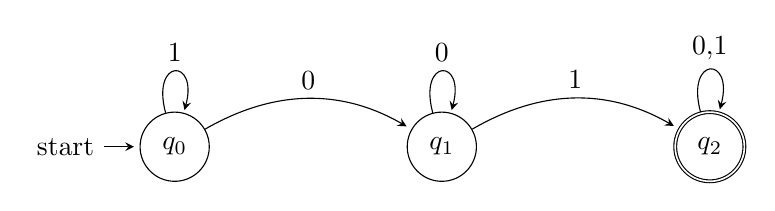
\begin{tikzpicture}[->, >=stealth, shorten >=2pt, auto, node distance=2.5cm]
% Estados
\node[state, initial] (q0) {$q_0$};
\node[state, right=of q0] (q1) {$q_1$};
\node[state, accepting, right=of q1] (q2) {$q_2$};
% Transiciones
\path
(q0) edge[bend left] node {0} (q1)
(q0) edge[loop above] node {1} ()
(q1) edge[loop above] node {0} ()
(q1) edge[bend left] node {1} (q2)
(q2) edge[loop above] node {0,1} ();
\end{tikzpicture}
\end{center}

\textbf{Tabla de transiciones:}
\begin{center}
\begin{tabular}{|c|c|c|}
\hline
 & 0 & 1 \\ \hline
$q_0$ & $q_1$ & $q_0$ \\ \hline
$q_1$ & $q_1$ & $q_2$ \\ \hline
$q_2$ & $q_2$ & $q_2$ \\ \hline

\end{tabular}
\end{center}

\textbf{Palabras aceptadas y palabras rechazadas}
\begin{center}
\begin{tabular}{|c|c|}
\hline
Aceptadas & No aceptadas \\
\hline
01 & 0 \\
001 & 10 \\
101 & 11 \\
010 & 100 \\
1101 & 111 \\
\hline
\end{tabular}
\end{center}

\section*{Ejercicio 4}
\textbf{Lenguaje:} Palabras que no contienen la subcadena “01”.  

\textbf{Tupla del AFD:}
\begin{itemize}
    \item $\Sigma = \{0,1\}$
    \item $Q = \{q_0, q_1, q_2, q_3\}$
    \item $q_0$ inicial
    \item $F = \{q_1, q_2\}$
\end{itemize}



\textbf{Tabla de transiciones:}
\begin{center}
\begin{tabular}{|c|c|c|}
\hline
 & 0 & 1 \\ \hline
$q_0$ & $q_1$ & $q_2$ \\ \hline
$q_1$ & $q_1$ & $q_3$ \\ \hline
$q_2$ & $q_1$ & $q_2$ \\ \hline
$q_3$ & $q_3$ & $q_3$ \\ \hline
\end{tabular}
\end{center}

\textbf{Diagrama del AFD:}
\begin{center}
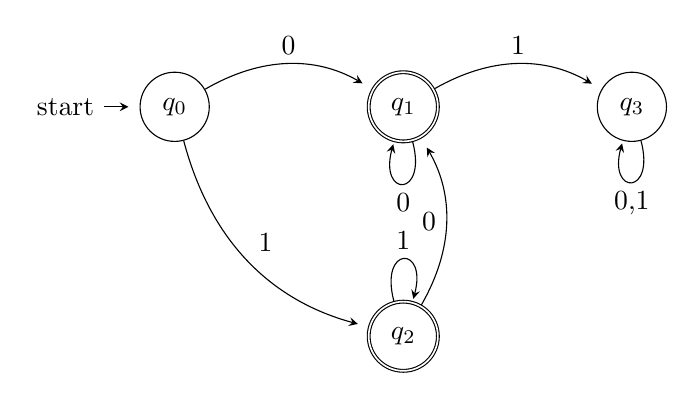
\begin{tikzpicture}[->, >=stealth, shorten >=4pt, auto, node distance=2cm]% Estados
\node[state, initial] (q0) {$q_0$};
\node[state, accepting, right=of q0] (q1) {$q_1$};
\node[state, accepting, below=of q1] (q2) {$q_2$};
\node[state, right=of q1] (q3) {$q_3$};

% Transiciones
\path
(q0) edge[bend left] node {0} (q1)
    edge[bend right] node {1} (q2)
(q1) edge[loop below] node {0} ()
    edge[bend left] node {1} (q3)
(q2) edge[loop above] node {1} ()
(q3) edge[loop below] node {0,1} ()
(q2) edge[bend right] node {0} (q1);
\end{tikzpicture}
\end{center}

\textbf{Palabras aceptadas y palabras rechazadas}
\begin{center}
\begin{tabular}{|c|c|}
\hline
Aceptadas & No aceptadas \\
\hline
0 & 01 \\
1 & 101 \\
00 & 001 \\
11 & 010 \\
000 & 1001 \\
\hline
\end{tabular}
\end{center}

\section*{Ejercicio 5}
\textbf{Lenguaje:} Palabras sobre $\Sigma = \{a,b,c\}$ que inician con “ac” o terminan con “ab”.  

\textbf{Tupla del AFD:}
\begin{itemize}
    \item $\Sigma = \{a,b,c\}$
    \item $Q = \{q_0, q_1, q_2, q_3, q_4, q_5\}$
    \item $q_0$ inicial
    \item $F = \{q_2, q_5\}$
\end{itemize}

\textbf{Diagrama del AFD:}
\begin{center}
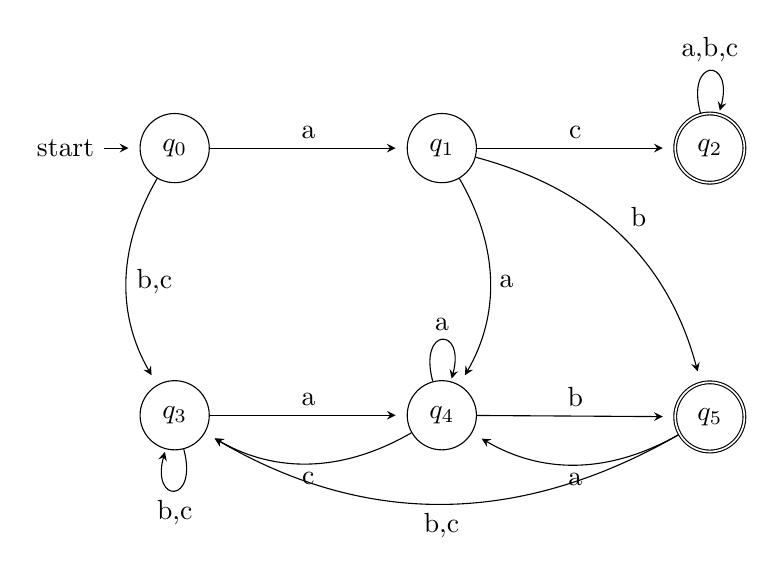
\begin{tikzpicture}[->, >=stealth, shorten >=4pt, auto, node distance=2.5cm]
% Estados
\node[state, initial] (q0) {$q_0$};
\node[state, right=of q0] (q1) {$q_1$};
\node[state, accepting, right=of q1] (q2) {$q_2$};
\node[state, below=of q0] (q3) {$q_3$};
\node[state, below=of q1] (q4) {$q_4$};
\node[state, accepting, below=of q2] (q5) {$q_5$};

% Transiciones
\path
(q0) edge node {a} (q1)
(q0) edge[bend right] node {b,c} (q3)
(q1) edge node {c} (q2)
(q1) edge[bend left] node {b} (q5)
(q1) edge[bend left] node {a} (q4)
(q4) edge[bend left] node {c} (q3)
(q4) edge[loop above] node {a} ()
(q2) edge[loop above] node {a,b,c} ()
(q3) edge node {a} (q4)
(q4) edge node {b} (q5)
(q3) edge[loop below] node {b,c} ()
(q5) edge[bend left] node {b,c} (q3)
(q5) edge[bend left] node {a} (q4);
\end{tikzpicture}
\end{center}

\textbf{Tabla de transiciones:}
\begin{center}
\begin{tabular}{|c|c|c|c|}
\hline
 & a & b & c \\ \hline
$q_0$ & $q_1$ & $q_3$ & $q_3$ \\ \hline
$q_1$ & $q_4$ & $q_5$ & $q_2$ \\ \hline
$q_2$ & $q_2$ & $q_2$ & $q_2$ \\ \hline
$q_3$ & $q_4$ & $q_3$ & $q_3$ \\ \hline
$q_4$ & $q_4$ & $q_5$ & $q_3$ \\ \hline
$q_5$ & $q_3$ & $q_3$ & $q_3$ \\ \hline
\end{tabular}
\end{center}

\textbf{Palabras aceptadas y palabras rechazadas}
\begin{center}
\begin{tabular}{|c|c|}
\hline
Aceptadas & No aceptadas \\
\hline
ac & a \\
acb & b \\
cab & c \\
bacab & ca \\
bab & abc \\
\hline
\end{tabular}
\end{center}

\section*{Ejercicio 6}
\textbf{Lenguaje:} Palabras que inician con “ac” y no terminan con “ab”.  

\textbf{Tupla del AFD:}
\begin{itemize}
    \item $\Sigma = \{a,b,c\}$
    \item $Q = \{q_0,q_1,q_2,q_3,q_4,q_5,q_6\}$
    \item $q_0$ inicial
    \item $F = \{q_3,q_4\}$
\end{itemize}

\textbf{Tabla de transiciones:}
\begin{center}
\begin{tabular}{|c|c|c|c|}
\hline
 & a & b & c \\ \hline
$q_0$ & $q_1$ & $q_3$ & $q_3$ \\ \hline
$q_1$ & $q_3$ & $q_3$ & $q_2$ \\ \hline
$q_2$ & $q_2$ & $q_2$ & $q_2$ \\ \hline
$q_3$ & $q_3$ & $q_4$ & $q_3$ \\ \hline
$q_4$ & $q_3$ & $q_4$ & $q_3$ \\ \hline
\end{tabular}
\end{center}

\textbf{Diagrama del AFD:}
\begin{center}
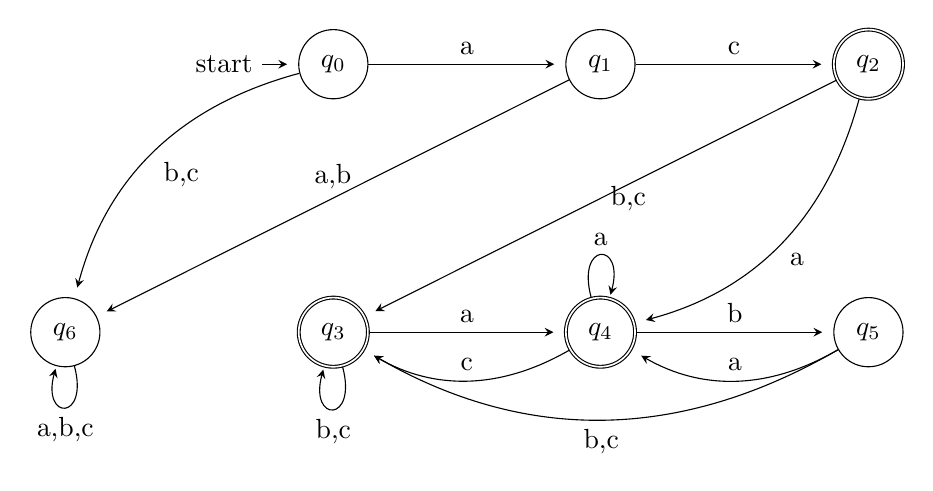
\begin{tikzpicture}[->, >=stealth, shorten >=4pt, auto, node distance=2.5cm]
% Estados
\node[state, initial] (q0) {$q_0$};
\node[state, right=of q0] (q1) {$q_1$};
\node[state, accepting, right=of q1] (q2) {$q_2$};
\node[state, accepting, below=of q0] (q3) {$q_3$};
\node[state, accepting, below=of q1] (q4) {$q_4$};
\node[state, below=of q2] (q5) {$q_5$};
\node[state, left=of q3] (q6) {$q_6$};
% Transiciones
\path
(q0) edge node {a} (q1)
(q0) edge[bend right] node {b,c} (q6)
(q1) edge node {c} (q2)
(q2) edge[ right] node {b,c} (q3)
(q2) edge[bend left] node {a} (q4)
(q4) edge[bend left] node[above] {c} (q3)
(q1) edge[left] node[above] {a,b} (q6)
(q4) edge[loop above] node {a} ()
(q3) edge node {a} (q4)
(q4) edge node {b} (q5)
(q3) edge[loop below] node {b,c} ()
(q6) edge[loop below] node {a,b,c} ()
(q5) edge[bend left] node {b,c} (q3)
(q5) edge[bend left] node[above] {a} (q4);
\end{tikzpicture}
\end{center}

\textbf{Palabras aceptadas y palabras rechazadas}

\section*{Ejercicio 7}
\textbf{Lenguaje:} Palabras que inician con “ac” o no terminan con “ab”.  

\textbf{Tupla del AFD:}
\begin{itemize}
    \item $\Sigma = \{a,b,c\}$
    \item $Q = \{q_0,q_1,q_2,q_3,q_4\}$
    \item $q_0$ inicial
    \item $F = \{q_2,q_3,q_4\}$
\end{itemize}

\textbf{Tabla de transiciones:}
\begin{center}
\begin{tabular}{|c|c|c|c|}
\hline
 & a & b & c \\ \hline
$q_0$ & $q_1$ & $q_3$ & $q_3$ \\ \hline
$q_1$ & $q_4$ & $q_5$ & $q_2$ \\ \hline
$q_2$ & $q_2$ & $q_2$ & $q_2$ \\ \hline
$q_3$ & $q_4$ & $q_3$ & $q_3$ \\ \hline
$q_4$ & $q_4$ & $q_5$ & $q_3$ \\ \hline
$q_5$ & $q_4$ & $q_3$ & $q_3$ \\ \hline
\end{tabular}
\end{center}

\textbf{Diagrama del AFD:}
\begin{center}
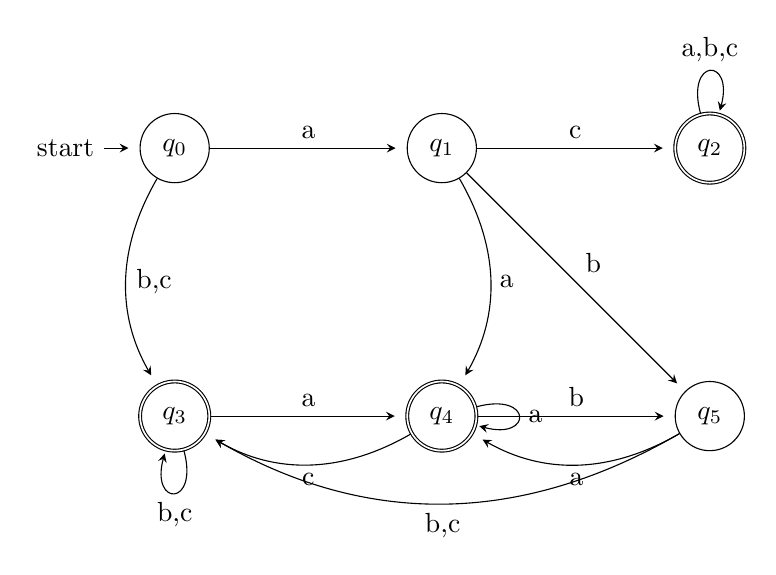
\begin{tikzpicture}[->, >=stealth, shorten >=4pt, auto, node distance=2.5cm]
% Estados
\node[state, initial] (q0) {$q_0$};
\node[state, right=of q0] (q1) {$q_1$};
\node[state, accepting, right=of q1] (q2) {$q_2$};
\node[state, accepting, below=of q0] (q3) {$q_3$};
\node[state, accepting, below=of q1] (q4) {$q_4$};
\node[state, below=of q2] (q5) {$q_5$};

% Transiciones
\path
(q0) edge node {a} (q1)
(q0) edge[bend right] node {b,c} (q3)
(q1) edge node {c} (q2)
(q1) edge[bend left] node {a} (q4)
(q1) edge node {b} (q5)
(q2) edge[loop above] node {a,b,c} ()
(q3) edge[loop below] node {b,c} ()
(q3) edge node {a} (q4)
(q4) edge[loop right] node {a} ()
(q4) edge node {b} (q5)
(q4) edge[bend left] node {c} (q3)
(q5) edge[bend left] node {b,c} (q3)
(q5) edge[bend left] node {a} (q4);
\end{tikzpicture}
\end{center}

\textbf{Palabras aceptadas y palabras rechazadas}
\begin{center}
\begin{tabular}{|c|c|}
\hline
Aceptadas & No aceptadas \\
\hline
ac & ab \\
acc & cab \\
bca & bab \\
ca & aab \\
aa & acab \\
\hline
\end{tabular}
\end{center}
\begin{center}
\begin{tabular}{|c|c|}
\hline
\end{tabular}
\end{center}


\section*{Ejercicio 8}
\textbf{Lenguaje:} Palabras que no inician con “ac” y no terminan con “ab”.  

\textbf{Tupla del AFD:}
\begin{itemize}
    \item $\Sigma = \{a,b,c\}$
    \item $Q = \{q_0,q_1,q_2,q_3,q_4\}$
    \item $q_0$ inicial
    \item $F = \{q_3,q_4\}$
\end{itemize}

\textbf{Tabla de transiciones:}
\begin{center}
\begin{tabular}{|c|c|c|c|}
\hline
 & a & b & c \\ \hline
$q_0$ & $q_1$ & $q_3$ & $q_3$ \\ \hline
$q_1$ & $q_3$ & $q_5$ & $q_2$ \\ \hline
$q_2$ & $q_2$ & $q_2$ & $q_2$ \\ \hline
$q_3$ & $q_4$ & $q_3$ & $q_3$ \\ \hline
$q_4$ & $q_4$ & $q_5$ & $q_3$ \\ \hline
$q_5$ & $q_4$ & $q_3$ & $q_3$ \\ \hline
\end{tabular}
\end{center}

\textbf{Diagrama del AFD:}
\begin{center}
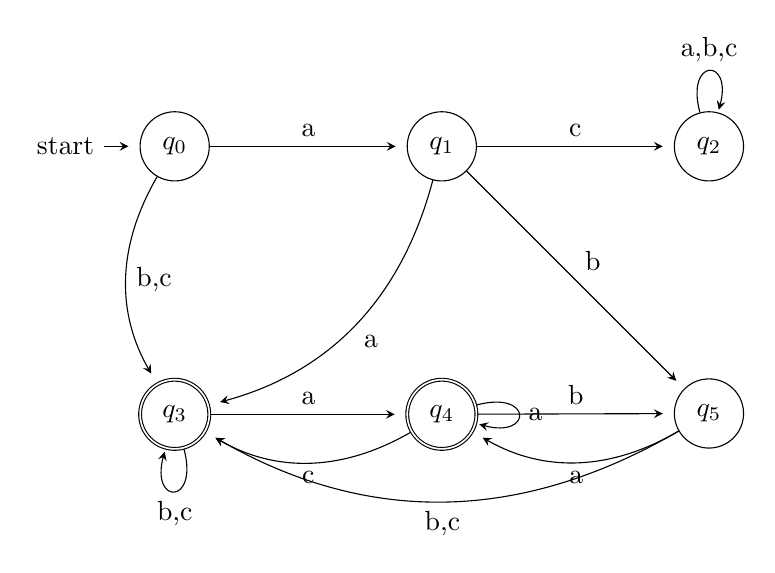
\begin{tikzpicture}[->, >=stealth, shorten >=4pt, auto, node distance=2.5cm]
% Estados
\node[state, initial] (q0) {$q_0$};
\node[state, right=of q0] (q1) {$q_1$};
\node[state, right=of q1] (q2) {$q_2$};
\node[state, accepting, below=of q0] (q3) {$q_3$};
\node[state, accepting, below=of q1] (q4) {$q_4$};
\node[state, below=of q2] (q5) {$q_5$};

% Transiciones
\path
(q0) edge node {a} (q1)
(q0) edge[bend right] node {b,c} (q3)
(q1) edge node {c} (q2)
(q1) edge[bend left] node {a} (q3)
(q1) edge node {b} (q5)
(q2) edge[loop above] node {a,b,c} ()
(q3) edge[loop below] node {b,c} ()
(q3) edge node {a} (q4)
(q4) edge[loop right] node {a} ()
(q4) edge node {b} (q5)
(q4) edge[bend left] node {c} (q3)
(q5) edge[bend left] node {b,c} (q3)
(q5) edge[bend left] node {a} (q4);
\end{tikzpicture}
\end{center}

\textbf{Palabras aceptadas y palabras rechazadas}
\begin{center}
\begin{tabular}{|c|c|}
\hline
Aceptadas & No aceptadas \\
\hline
baa & ac \\
ca & ab \\
cbc & acb \\
bbc & acc \\
aac & acab \\
\hline
\end{tabular}
\end{center}
\begin{center}
\begin{tabular}{|c|c|}
\hline
Aceptadas & No aceptadas \\
\hline
baa & ac \\
ca & acb \\
cbc & acc \\
bbc & aca \\
aac & acab \\
\hline
\end{tabular}
\end{center}


\section*{Ejercicio 9 (AFND)}
\textbf{Lenguaje:} Palabras que no contienen la subcadena "01".  

\textbf{Tupla del AFND:}
\begin{itemize}
    \item $\Sigma = \{0,1\}$
    \item $Q = \{q_0,q_1,q_2\}$
    \item $q_0$ inicial
    \item $F = \{q_0,q_1\}$
\end{itemize}

\textbf{Tabla de transiciones:}
\begin{center}
\begin{tabular}{|c|c|c|}
\hline
 & 0 & 1 \\ \hline
$q_0$ & $\{q_1\}$ & $\{q_0\}$ \\ \hline
$q_1$ & $\{q_1\}$ & $\{q_2\}$ \\ \hline
$q_2$ & $\{q_2\}$ & $\{q_2\}$ \\ \hline
\end{tabular}
\end{center}

\textbf{Diagrama del AFND:}
\begin{center}
\begin{tikzpicture}[->, >=stealth, shorten >=4pt, auto, node distance=2.5cm]
% Estados
\node[state, initial, accepting] (q0) {$q_0$};
\node[state, accepting, right=of q0] (q1) {$q_1$};
\node[state, below right=of q1] (q2) {$q_2$};

% Transiciones
\path
(q0) edge[bend left] node {0} (q1)
(q0) edge[loop above] node {1} ()
(q1) edge[loop above] node {0} ()
(q1) edge node {1} (q2)
(q2) edge[loop right] node {0,1} ();
\end{tikzpicture}
\end{center}

\textbf{Palabras aceptadas y palabras rechazadas}
\begin{center}
\begin{tabular}{|c|c|}
\hline
Aceptadas & No aceptadas \\
\hline
0 & 01 \\
1 & 001 \\
00 & 101 \\
11 & 0101 \\
111 & 1011 \\
\hline
\end{tabular}
\end{center}

\section*{Ejercicio 10 (AFND)}
\textbf{Lenguaje:} Palabras que inician con “ac” y terminan con “ab”.  

\textbf{Tupla del AFND:}
\begin{itemize}
    \item $\Sigma = \{a,b,c\}$
    \item $Q = \{q_0,q_1,q_2,q_3,q_4\}$
    \item $q_0$ inicial
    \item $F = \{q_4\}$
\end{itemize}

\textbf{Tabla de transiciones:}
\begin{center}
\begin{tabular}{|c|c|c|c|}
\hline
 & a & b & c \\ \hline
$q_0$ & $\{q_1\}$ & $\emptyset$ & $\emptyset$ \\ \hline
$q_1$ & $\emptyset$ & $\emptyset$ & $\{q_2\}$ \\ \hline
$q_2$ & $\{q_2,q_3\}$ & $\{q_2\}$ & $\{q_2\}$ \\ \hline
$q_3$ & $\emptyset$ & $\{q_4\}$ & $\emptyset$ \\ \hline
$q_4$ & $\emptyset$ & $\emptyset$ & $\emptyset$ \\ \hline
\end{tabular}
\end{center}

\textbf{Diagrama del AFND:}
\begin{center}
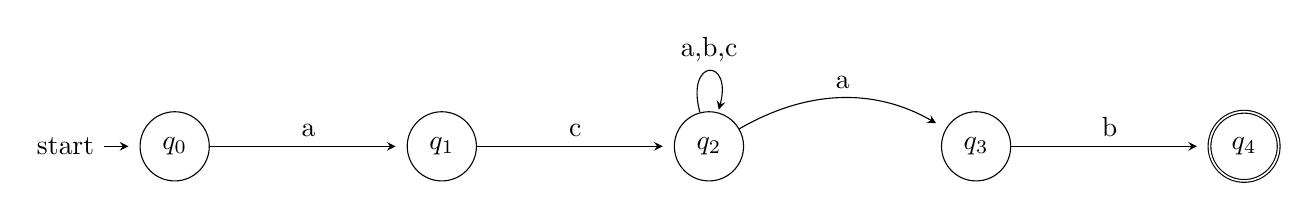
\begin{tikzpicture}[->, >=stealth, shorten >=4pt, auto, node distance=2.5cm]
% Estados
\node[state, initial] (q0) {$q_0$};
\node[state, right=of q0] (q1) {$q_1$};
\node[state, right=of q1] (q2) {$q_2$};
\node[state, right=of q2] (q3) {$q_3$};
\node[state, accepting, right=of q3] (q4) {$q_4$};

% Transiciones
\path
(q0) edge node {a} (q1)
(q1) edge node {c} (q2)
(q2) edge[loop above] node {a,b,c} ()
(q2) edge[bend left] node {a} (q3)
(q3) edge node {b} (q4);
\end{tikzpicture}
\end{center}

\textbf{Palabras aceptadas y palabras rechazadas}
\begin{center}
\begin{tabular}{|c|c|}
\hline
Aceptadas & No aceptadas \\
\hline
acab & ac \\
acabcab & acc \\
acbab & acbc \\
acaabab & acba \\
accbcab & abac \\
\hline
\end{tabular}
\end{center}

\end{document}
